% % ----------------------------------------------------------------------- %
% % Arquivo: 3-cenario-IFSC.tex
% % ----------------------------------------------------------------------- %

% \chapter{Estudo de Caso: Infraestrutura de Serviços do IFSC}
% \label{c_cenario}

% Após conversas com servidores da \ac{CTIC} do \ac{IFSC} câmpus São José e pesquisas realizadas em documentos disponíveis em portais da instituição percebeu-se que há um movimento emergente em setores do \ac{IFSC} para implantação de políticas de \ac{TI} eficientes e condizentes com a realidade da instituição. Há também discussões sobre os serviços atualmente fornecidos por cada câmpus da instituição e sobre como melhorar a disponibilidade e eficiência dos serviços oferecidos através do \textit{data center} mantido pela Reitoria do \ac{IFSC}, onde a infraestrutura de serviços da instituição é centralizada.

% Por este motivo, é necessário contextualizar o presente estado das políticas de \ac{TI} e infraestrutura do \ac{IFSC} para que o sistema distribuído proposto neste trabalho possa ser melhor entendido e justificado. A seguir é feita uma discussão sobre as políticas de \ac{TI} do \ac{IFSC}, os pontos positivos da centralização da infraestrutura e as deficiências do modelo de infraestrutura adotados pela instituição.

% % ----------------------------------------------------------------------- %
% \section{Política de TI do IFSC}

% Nos últimos anos o \ac{IFSC} tem se preocupado com suas políticas de governança de \ac{TI}. Em 2015, por exemplo, diversas normas e políticas foram adotadas pelo \ac{IFSC} em relação ao uso de recursos pelos discentes e docentes dos câmpus da instituição \cite{dticpoliticas}. Em 2017 foi criada a Coordenadoria de Governança de \ac{TI}, responsável por responder pelos processos de compras de \ac{TI}, planejamento e governança \cite{pdti2018}. A estrutura organizacional atual da \ac{TIC} do \ac{IFSC} é exibida na \autoref{organizacaoIFSC}, e a descrição das funções de cada departamento é descrita na Resolução CONSUP nº 12, de 24 de abril de 2017 \cite{pdti2018}.

% \begin{figure}[!htpb]
% 	\centering
% 	\caption{Estrutura institucional da TIC do IFSC}
%     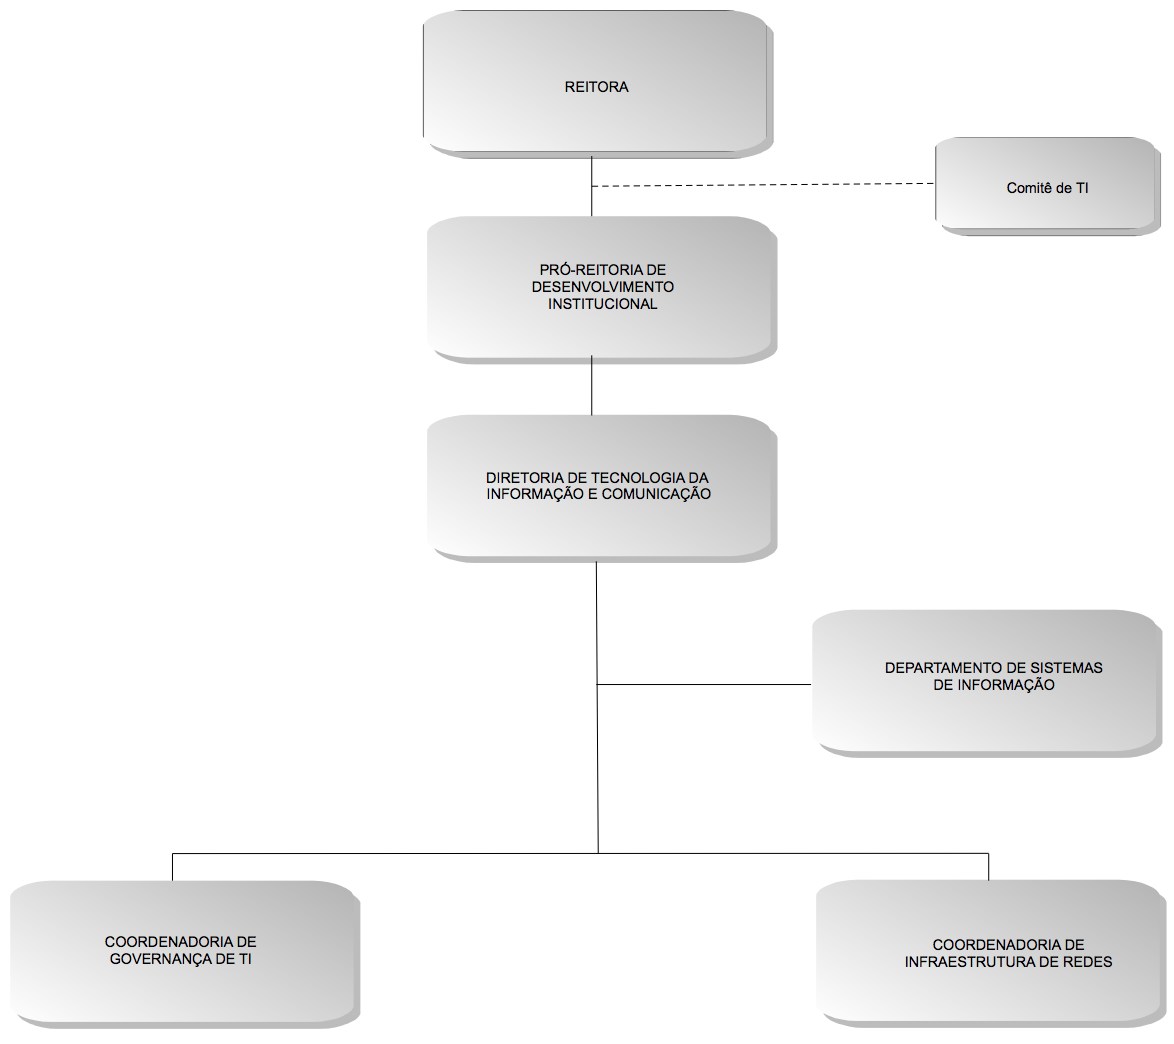
\includegraphics[width=15cm]{TCC/figuras/3-cenario/OrganogramaIFSC}
    
% 	Fonte: Extraído de \cite{pdti2017}
%  	\label{organizacaoIFSC}
% \end{figure}

% Embora haja esforço para estabelecimento de novas políticas, normas e procedimentos de \ac{TI} dentro da instituição, ainda há muito a ser feito. A \ac{UFSC}, por exemplo, já possui suas políticas e procedimentos de \ac{TI} definidos e em constante aprimoramento. A instituição já está ofertando acesso a serviços em nuvem à comunidade acadêmica \cite{seticNuvem} e possui um portal público onde são registradas manutenções na rede e em serviços ofertados à comunidade acadêmica \cite{seticUFSC}. Além disso, a matriz de responsabilidade da instituição define as responsabilidades atribuídas a membros da \ac{SeTIC}, o que também contribui com a transparência e organização do setor \cite{matrizUFSC}. O reconhecimento da organização e gestão dos setores de \ac{TI} da \ac{UFSC} é percebido no cálculo do perfil de governança de \ac{TI} da instituição, realizado pelo \ac{TCU}. Este índice vai de 0 a 1, sendo que quanto maior o índice, melhor a condução das políticas de \ac{TI} da instituição.  Em 2016 o índice alcançado pela \ac{UFSC} foi de 0,61 (intermediário), enquanto o índice obtido pelo \ac{IFSC} foi de 0,38 (básico) \cite{igovti}. A média das instituições avaliadas é de 0,49 com desvio padrão de 0,18.

% Existem iniciativas dentro da instituição para aumentar a transparência dos setores de \ac{TI}. A \ac{CTIC} do câmpus São José, por exemplo, já compartilha publicamente os códigos utilizados para manutenção e implantação de serviços \cite{github-sj} e também disponibiliza acesso a plataforma de gestão de seus projetos \cite{trello-sj}. A iniciativa do câmpus São José mostra como políticas de \ac{TI} e transparência são emergentes dentro da instituição. Entretanto, o interesse na implantação de tais políticas também deve partir de cargos de coordenadoria e de departamentos da alta hierarquia, os quais devem se preocupar com o cenário global de transparência e organização da instituição. É importante ressaltar que a implantação de políticas de \ac{TI} é um processo demorado e trabalhoso, mas que após a implantação de tais políticas a gestão de recursos da instituição é facilitada e mais eficiente. O \ac{GED}, por exemplo, é um tópico recorrente em cada edição do \ac{PDTI} desde 2011, sendo seu estado de execução constantemente descrito como \textit{em execução} {\color{blue}(IFSC, 2011, 2013, 2014, 2016, 2017, 2018b)}. Após implantado, o sistema de gestão de documentos eletrônicos deverá permitir acesso a cópias digitalizadas de todos os documentos da instituição, aumentando a transparência do \ac{IFSC} e facilitando o fornecimento de documentos ao público. É importante ressaltar que, de acordo com a Portaria nº 315, de 4 de abril de 2018, o \ac{IFSC} possui até abril de 2020 para converter para o meio digital os ``documentos e informações que compõem o acervo acadêmico, independente da fase em que se encontrem ou de sua destinação final'' \cite{portaria315}. Esta é, portanto, uma discussão que também é realizada em outras instituições de ensino.

% Espera-se que o sistema proposto neste trabalho juntamente com as propostas de infraestrutura da \ac{CTIC} do câmpus São José sejam não apenas implantados no futuro, mas que também tragam mais atenção a discussões referentes a governança e políticas de \ac{TI} dentro da instituição e resolvam algumas das deficiências do modelo atual.


% % ----------------------------------------------------------------------- %
% \section{Pontos Positivos do Modelo Atual}

% Entre os pontos positivos do modelo de infraestrutura de serviços atual do \ac{IFSC} encontram-se a facilidade na administração dos serviços ofertados e armazenamento de dados, os quais estão localizados em apenas um \textit{data center}.

% Também é importante ressaltar que os funcionários dos departamentos de \ac{TIC} dos câmpus do \ac{IFSC} possuem diferentes formações e especialidades. Logo, o modelo centralizado permite que os funcionários que possuam maior capacitação para manutenção do sistema possam estar concentrados nestas funções. Expandir a infraestrutura para outros câmpus significaria a necessidade de treinamento das equipes de \ac{TIC}, o que pode ser demorado e custoso para a instituição.

% O modelo centralizado e topologia vertical do sistema podem ser onerosos, mas a alta qualidade do \textit{hardware} utilizado fornece confiabilidade ao sistema. Além disso, as garantias e assistências técnicas contratadas para tal \textit{hardware} permitem que a manutenção de tais equipamentos sejam agilizada devido as especialidades das empresas de manutenção contratadas.

% O atual funcionamento do sistema permite também que novos serviços possam ser mais facilmente implementados, enquanto uma remodelagem do sistema resultaria em um grande movimento para migração de serviços e verificação de compatibilidade dos serviços atuais com uma nova infraestrutura.

% % ----------------------------------------------------------------------- %
% \section{Cenário Ideal}

% O cenário ideal de infraestrutura em nuvem do \ac{IFSC} consiste em uma infraestrutura de alta disponibilidade, baixo custo financeiro, alto poder de processamento, fácil manutenção e gerenciamento, e que possa ser futuramente integrada a outras nuvens e serviços externos a instituição. Também faz parte do cenário ideal a implementação de um \textit{data center} horizontal e distribuído, concentrando a redundância da infraestrutura em \textit{software} ao invés de em \textit{hardware}, dispensando assim dispositivos complexos e proprietários que tornem a instituição dependente de terceiros tanto na instalação quanto na manutenção destes dispositivos. Os aplicativos utilizados devem ser livres e utilizar padrões abertos, permitindo assim que sejam utilizados sem restrições de licenças e possam ser facilmente integrados com outras nuvens. Já a infraestrutura deve ser distribuída e possuir distribuição de carga na utilização e acesso de serviços e dados. Esta nuvem deve continuar oferecendo os serviços que já são oferecidos à comunidade acadêmica atual e implementar ainda mais serviços, como utilização remota de aplicativos disponíveis apenas nas unidades físicas da instituição, por exemplo. Todas estas características são sugeridas para que o \ac{IFSC} possua uma infraestrutura tolerante a falhas, eficaz e facilmente escalável, permitindo assim que a comunidade acadêmica seja amplamente atendida e não vivencie interrupções de serviços.

% Além destes requisitos também é necessário que os funcionários de \ac{TI} dos câmpus do \ac{IFSC} sejam capacitados para operar e manter este sistema, delegando assim funções específicas para  membros específicos do setor. Considerando que todos os serviços acadêmicos (tanto administrativos quanto de ensino) seriam migrados para esta infraestrutura, é necessário, portanto, que cada câmpus possua pelo menos um responsável pela manutenção da infraestrutura e serviços ofertados neste câmpus.

% Com a expansão da infraestrutura de serviços e aumento do poder de processamento do sistema também é possível oferecer a maior parte dos serviços utilizados pela instituição em nuvem, dispensando assim a necessidade de utilização de aplicativos que necessitem de processamento local, fato que possibilitaria a troca de computadores por terminais mais simples para acesso à nuvem da instituição, haja vista que o processamento ocorre remotamente, e não localmente.

% % ----------------------------------------------------------------------- %
% \section{Deficiências do Modelo}

% Atualmente, as infraestruturas dos câmpus do \ac{IFSC} atuam de forma independente e utilizam alguns serviços fornecidos e mantidos pela Reitoria do \ac{IFSC}, a qual planeja continuar com o processo de ``\textit{centralização de infraestrutura e serviços no data center da reitoria}'' \cite{pdti2018}. Os demais câmpus da rede possuem suas infraestruturas individuais, sobretudo projetadas para atenderem às suas necessidades. O câmpus do \ac{IFSC} de São José, por exemplo, fornece acesso através de \ac{SSH} para as aplicações Octave e MATLAB, as quais são utilizadas pelos alunos dos cursos de telecomunicações \cite{github-sj-servicos}.

% De acordo com as classificações de \textit{Tiers} de \textit{data centers} realizados pela \citeonline{tierCPD} e a partir de conversas com funcionários do departamento de \ac{CTIC} do \ac{IFSC} câmpus São José, a infraestrutura do \textit{data center} mantido na Reitoria da instituição possivelmente se encaixa entre as classificações de \textit{Tier} I e II. Diz-se possivelmente pois não há documentação publicamente acessível que descreva tanto os equipamentos utilizados ou a infraestrutura física do \textit{data center}. O motivo pelo qual o \textit{data center} não se encaixa na categoria de \textit{Tier} II é porque não há redundância e replicação geográfica dos dados e serviços oferecidos (georreplicação), o que aumenta a probabilidade de pontos únicos de falha no sistema (\ac{SPOF}). Um exemplo de serviço mantido pela Reitoria que causaria grande transtorno caso apresente falhas é o acesso ao serviço \ac{LDAP} do \ac{IFSC}. Este serviço centraliza a autenticação de serviços \cite{pdti2011} e é usado por todos os sistemas de informação da instituição \cite{mello-helios}. Caso haja interrupção neste serviço, não será possível autenticar-se em redes sem fio de todos os câmpus, portais institucionais e afins.

% Uma alternativa para resolver o problema de redundância e replicação de dados e serviços da instituição é a integração entre infraestruturas dos câmpus, o que ofereceria redundância de dados e serviços para toda a rede do \ac{IFSC}. Apesar desta alternativa, o \ac{IFSC} planeja continuar investindo na centralização de serviços. De acordo com a Resolução CONSUP nº 12, de 24 de abril de 2017 \cite{pdti2017}, planejava-se gastar R\$ 620.000,00 na otimização de recursos físicos, de pessoal e financeiro \textbf{centralizando} os serviços de redes na Grande Florianópolis, além da construção de infraestrutura mínima nos câmpus do interior. É importante ressaltar que o documento de fato se refere à Grande Florianópolis, abrangendo assim os três maiores câmpus da instituição: São José, Florianópolis e Continente. Entretanto, esta mesma resolução não descreve como esta verba é distribuída entre os câmpus e nem descreve quais recursos são necessários para otimização da estrutura. Também não é descrita como é realizada esta centralização, e logo não é possível saber se há integração entre as infraestruturas dos câmpus da Grande Florianópolis ou concentração de investimento apenas na infraestrutura da Reitoria.

% Também é importante ressaltar que a infraestrutura física da Reitoria (onde os serviços são atualmente concentrados) é limitada, não tendo sido (pelo menos a princípio) projetada para atuar como um grande \textit{data center} (como dito anteriormente, não foi possível localizar as plantas baixa, elétrica ou hidráulica nos portais da instituição para analisar a infraestrutura física do \textit{data center}). Por este motivo, a escalabilidade do sistema é sobretudo vertical, ou seja, para melhorar o desempenho do sistema é necessário adquirir servidores e \textit{storages} que possuam mais recursos que os atuais. Isto faz com que sejam gastos mais recursos financeiros que o ideal, haja vista que não é possível escalar o sistema horizontalmente através da topologia \ac{ToR}, simplesmente adicionando nós de processamento e armazenamento mais simples e de menor custo ao \textit{data center}. Os custos elevados de utilização da topologia vertical não se aplicam apenas à compra do equipamento, mas também à aquisição de serviços de instalação e manutenção dos dispositivos, pois estes são de fabricantes que possuem tecnologia proprietária e não podem ser mantidos apenas por servidores do \ac{IFSC}. De acordo com a Resolução CONSUP nº 03, de 26 de fevereiro de 2018 \cite{pdti2018}, o \ac{IFSC} orçou gastar R\$ 119.960,00 em serviços de instalação, configuração e garantia de \textit{storage} em 2018. Se infraestrutura da rede do \ac{IFSC} fosse integrada, seria possível adicionar nós de processamento e armazenamento em diversos câmpus, aproveitando a estrutura física de todos os câmpus, melhorando o desempenho global do sistema e potencialmente diminuindo o custo de expansão e melhoria do sistema.
